Consider a 3SAT problem with m clauses $c_j$ and n variables $x_i$. We construct a single source-sink congestion game and demonstrate that if in this game there exists a NE with the cost of 0 then the the 3SAT formula can be satisfied.

Consider the following graph $G$. We introduce a node $C_j$ for every clause $c_j$ and three nodes $A_i,X_i,not\ X_i$ for every variable $x_i$.

We introduce two type of edges:

Type 1 edges: cost is 0 for $x\leq1$ and $1$ for $x>1$

Type 2 edges: cost is 0 for $x=2$ and $1$ for $x\neq 2$

Nodes $A_i$ are connected to the sink with with type 1 edges. Nodes $A_i$ are connected to $X_i$ and $not\ X_i$ with edges of cost 0. Variable node $X_i$ ($\not\ X_i$) is connected to clause node $C_j$ if $x_i$ is in clause $c_j$ (if $\neg x_i$ is in $c_j$). Nodes $c_j$ are also connected to the source with type 1 edges and to the sink with type 2 edges. (see the diagram)

There are $n+m$ agents.

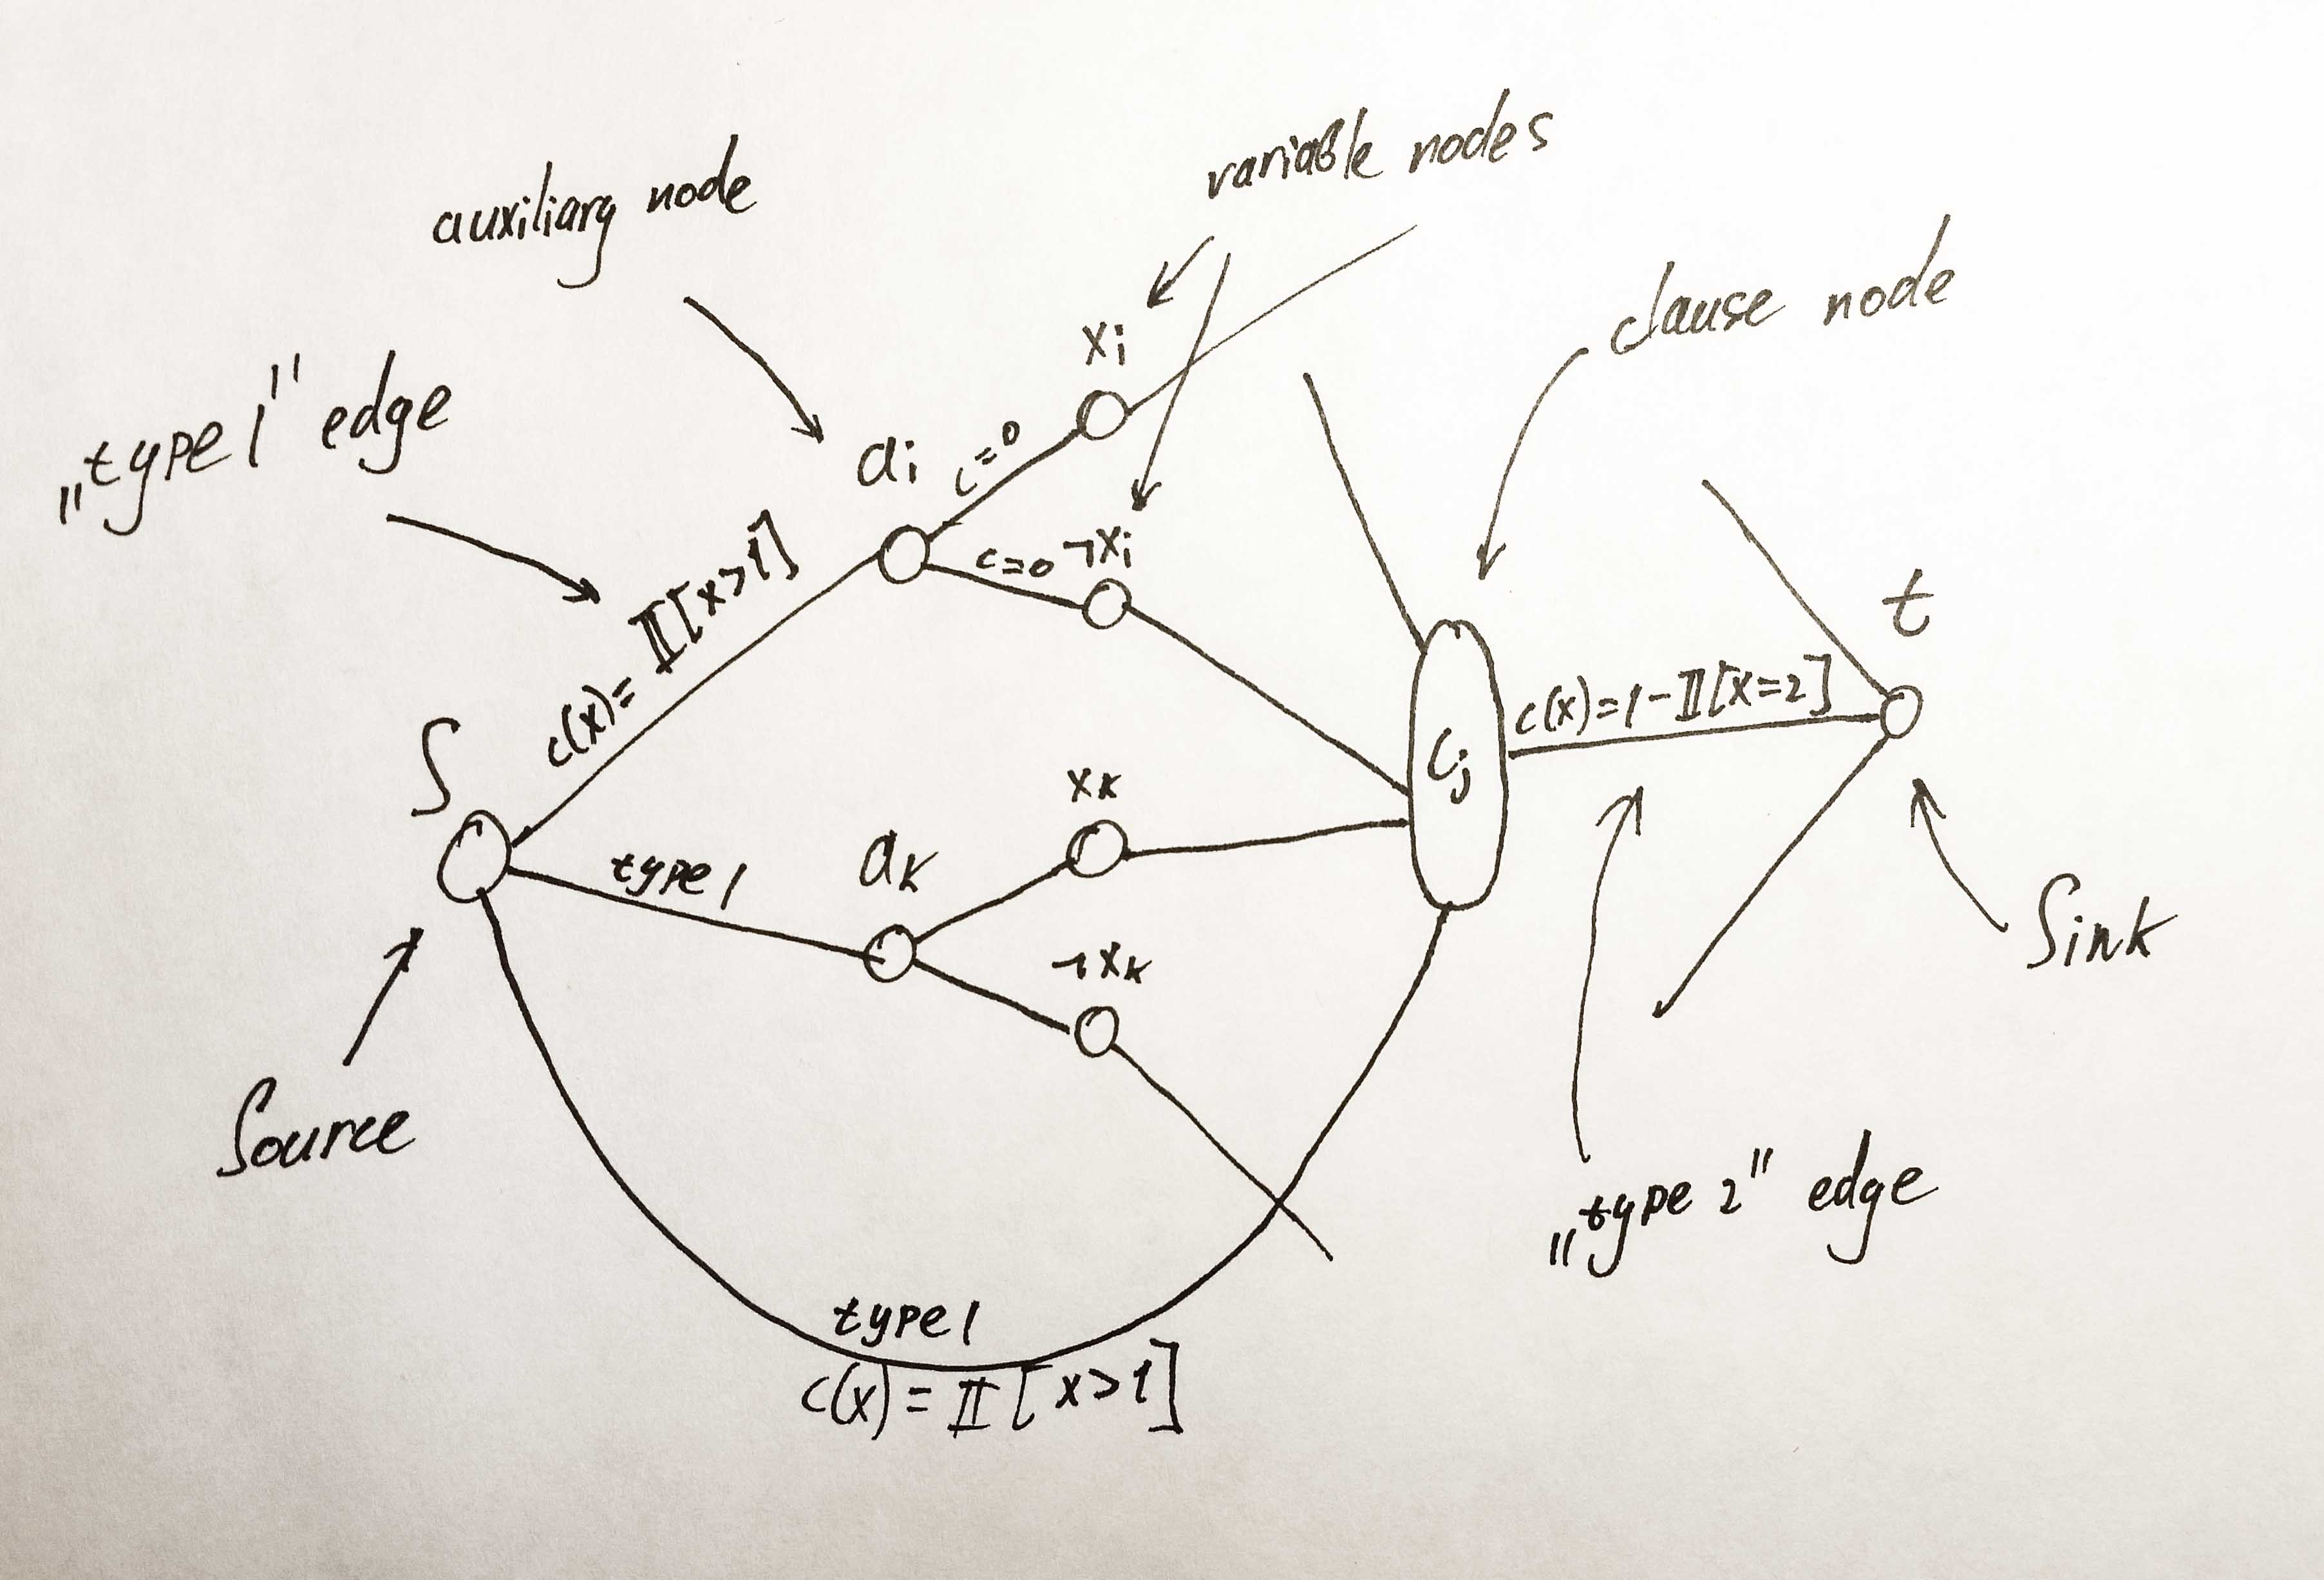
\includegraphics[scale=0.5]{1.jpg}

\uline{\textbf{Lemma}} If original 3SAT is satisfiable, $G$ has a NE of cost 0.

\uline{\textbf{Lemma}} If  $G$ has a NE of cost 0, original 3SAT is satisfiable.

\uline{\textbf{Theorem}} Finding best NE in a congestion game is NP hard.


\textif{Proof.} Notice that constructing $G$ is a polynomial in $n,m$ task. The statement now follows from previous lemmas.

